\documentclass{article}
\usepackage{graphicx} % Required for inserting images
\usepackage[margin=1in]{geometry}
\usepackage{amsmath}
\usepackage{amsthm}
\usepackage{amssymb}
\usepackage{amsfonts}
\usepackage{enumitem}
\usepackage{verbatim}
\usepackage{xcolor}

\title{Homework 1: Report}
\author{Dante Buhl}
\date{Feb. $26^{th}$ 2024}


\DeclareMathOperator{\cond}{cond}
\DeclareMathOperator{\vecspan}{span}

\begin{document}

\newcommand{\bs}[1]{\boldsymbol{#1}}
\newcommand{\bmp}[1]{\begin{minipage}{#1\textwidth}}
\newcommand{\emp}{\end{minipage}}
\newcommand{\R}{\mathbb{R}}
\newcommand{\C}{\mathbb{C}}
\newcommand{\N}{\mathcal{N}}
\newcommand{\I}{\mathrm{I}}
\newcommand{\K}{\bs{\mathrm{K}}}
\newcommand{\m}{\bs{\mu}_*}
\newcommand{\s}{\bs{\Sigma}_*}
\newcommand{\dt}{\Delta t}
\newcommand{\tr}[1]{\text{Tr}(#1)}
\newcommand{\Tr}[1]{\text{Tr}(#1)}

\maketitle

\section*{Problem 1: }
\begin{enumerate}[label=\alph*)]


    \item Derive the four-point finite-difference backward differentiation formula (BDF3) ap-
proximation of the first derivative of $f$. 
    \begin{proof}
        \begin{align}
            f'(x_j) &\simeq \frac{11f(x_j) - 18f(x_{j-1}) + 9f(x_{j-2}) - 2f(x_{j-3})}{6\Delta x}
        \end{align}

    We start with the polynomial approximation $f(x) \simeq \prod_4f(x)$ as a 4 point polynomial interpolation with lagranian polynomials. Also note that I will be using the notation of $x_0 = x_{j-3}$, $ x_1 = x_{j-2}$, $x_2 = x_{j-1}$, $x_3 = x_j$. 
        \begin{align}
            f(x) &\simeq \prod_4f(x) = f(x_0) l_0(x) + f(x_1) l_1(x) + f(x_2) l_2(x) + f(x_3)l_3(x) \\
            \frac{df}{dx} &\simeq \frac{d\prod_4f}{dx} = f(x_0) l_0'(x) + f(x_1) l_1'(x) + f(x_2) l_2'(x) + f(x_3)l_3'(x)
        \end{align}

        We will now look at $f'(x_3) \simeq \frac{d\prod_4f}{dx}(x_3)$. To reduce its complexity we look at the individual components $l_i'(x_3)$ first. For $i \neq 3$ we have, 
        \begin{align}
            l_i'(x) &= \left(\prod_{j \neq i}\frac{1}{x_i - x_j}\right)\frac{d \prod_{j \neq i}(x - x_j)}{dx} \\
            l_i'(x) &= \left(\prod_{j \neq i}\frac{1}{x_i - x_j}\right) \sum_{j\neq i}\prod_{k \neq i, j} (x - x_k) \\
            i \neq 3, \quad l_i'(x_3) &= \left(\prod_{j \neq i}\frac{1}{x_i - x_j}\right) \prod_{k \neq i, 3} (x_3 - x_k) \\
            i = 3, \quad l_i'(x_3),  &= \sum_{j \neq 3} \frac{1}{x_3 - x_j}
        \end{align}

        Finally we assume an evenly spaced grid. That is, $x_3 = x_0 + 3\Delta x$, $x_3 = x_1 + 2\Delta x$, and $x_3 = x_2 + \Delta x$. 

        \begin{align}
            l_0'(x_3) &= \frac{(2\Delta x)(\Delta x)}{(-3\Delta x)(-2\Delta x)(-\Delta x)} = -\frac{1}{3\Delta x} \\
            l_1'(x_3) &= \frac{(3\Delta x)(\Delta x)}{(\Delta x)(-2\Delta x)(-\Delta x)} = \frac{3}{2\Delta x}\\
            l_2'(x_3) &= \frac{(3\Delta x)(2\Delta x)}{(\Delta x)(2\Delta x)(-\Delta x)} = -\frac{3}{\Delta x}\\
            l_3'(x_3) &= \left(\frac{1}{3\Delta x} + \frac{1}{2\Delta x} + \frac{1}{\Delta x}\right) = \frac{11}{6\Delta x}
        \end{align}

        \begin{align}
            f'(x_3) &\simeq f(x_0) l_0'(x_3) + f(x_1) l_1'(x_3) + f(x_2) l_2'(x_3) + f(x_3)l_3'(x_3) \\
                          &\simeq -\frac{f(x_0)}{3\Delta x} + \frac{3f(x_1)}{2\Delta x} - \frac{3f(x_2)}{\Delta x} + \frac{11f(x_3)}{6\Delta x} \\
                          &\simeq \frac{11f(x_3) - 18f(x_2)+ 9f(x_1)-2f(x_0)}{6\Delta x}
\
        \end{align}
    \end{proof}

    \item Prove that (1) converges with order 3 in $\Delta x$ to the analytical derivative $f'(x_j)$.

    \begin{proof}
    
        We begin this proof using taylor polynomial approximations for $f(x)$ centered at $x_3$ (Note: $h.o.t.$ indicates ``higher order terms'').
        
        \begin{align}
            f(x_2) &\simeq f(x_3) - f'(x_3)\Delta x + \frac{f''(x_3)\Delta x^2}{2} - \frac{f'''(x_3) \Delta x^3}{6} + \frac{f''''(x_3)\Delta x^4}{24} + h.o.t. \\
            f(x_1) &\simeq f(x_3) - 2f'(x_3)\Delta x + \frac{4f''(x_3)\Delta x^2}{2} - \frac{8f'''(x_3) \Delta x^3}{6} + \frac{16f''''(x_3)\Delta x^4}{24} + h.o.t. \\
            f(x_0) &\simeq f(x_3) - 3f'(x_3)\Delta x + \frac{9f''(x_3)\Delta x^2}{2} - \frac{27f'''(x_3) \Delta x^3}{6} + \frac{81f''''(x_3)\Delta x^4}{24} + h.o.t. 
        \end{align}

        \begin{align}
            \frac{f(x_2) - f(x_3)}{\Delta x} + f'(x_3) &\simeq \frac{f''(x_3)\Delta x}{2} - \frac{f'''(x_3) \Delta x^2}{6} + \frac{f''''(x_3)\Delta x^3}{24} + h.o.t. \\
            \frac{f(x_1) - f(x_3)}{2\Delta x} + f'(x_3) &\simeq \frac{2f''(x_3)\Delta x}{2} - \frac{4f'''(x_3) \Delta x^2}{6} + \frac{8f''''(x_3)\Delta x^3}{24} + h.o.t. \\
            \frac{f(x_0) - f(x_3)}{3\Delta x} + f'(x_3) &\simeq \frac{3f''(x_3)\Delta x}{2} - \frac{9f'''(x_3) \Delta x^2}{6} + \frac{27f''''(x_3)\Delta x^3}{24} + h.o.t. 
        \end{align}

        Notice that we have 3 equations, and wish to eliminate all terms with second and third derivatives. We now use some basic linear algebra in order to eliminate the desired terms. We will express the desired equation as $A(18) + B(19) + C(20)$, where $A, B, C$ are scalar multipliers. The resulting system of equations is, 
    \begin{align}
        \left[ \begin{array}{c c c} 1 & 1 & 1 \\ 1 & 2 & 3 \\ 1 & 4 & 9 \end{array} \right] \left[ \begin{array}{c} A  \\ B \\ C\end{array}\right] &= \left[\begin{array}{c} 1 \\ 0 \\ 0\end{array}\right]
    \end{align}
    This system has solution, $A = 3$, $B = -3$, $C = 1$. We obtain a new equation using these scalar coefficients. 
    \begin{align}
        \begin{split}
            3\frac{f(x_2) - f(x_3)}{\Delta x} -3\frac{f(x_1) - f(x_3)}{2\Delta x} +  \frac{f(x_0) - f(x_3)}{3\Delta x} + f'(x_3)  \simeq \\ f''''(x_3)\Delta x^3 \left(\frac{3}{24} -  \frac{24}{24} + \frac{27}{24}\right) + h.o.t. 
        \end{split}
    \end{align}
    \begin{align}
            \frac{18f(x_2) - 18f(x_3) - 9f(x_1) + 9f(x_3) + 2f(x_0) - 2f(x_3)}{6\Delta x} + f'(x_3)  \simeq \frac{f''''(x_3)\Delta x^3}{4} + h.o.t. \\
            f'(x_3) - \frac{11f(x_3) - 18f(x_2)  + 9f(x_1) -  2f(x_0)}{6\Delta x}  \simeq \frac{f''''(x_3)\Delta x^3}{4} + h.o.t. \\
            \left\lVert f'(x_3) - \frac{11f(x_3) - 18f(x_2)  + 9f(x_1) -  2f(x_0)}{6\Delta x}\right\rVert_{\infty} \simeq \left\lVert\frac{f''''(x_3)\Delta x^3}{4}\right\rVert_{\infty} = O(\Delta x^3)
    \end{align}
        Thus, this derivative approximation converges cubically with $\Delta x$.

    \end{proof}
        
    
    \item Show numerically that (1) converges with order 3 by applying it to the periodic
function, 
        \[
            f(x) = \log(2 + \sin(2\pi x))
        \]
    \begin{proof}
    
        We first look at the analytical derivative. 
        \[
            f'(x) = \frac{1}{\ln(10)(2 + \sin(2\pi x))}(2\pi\cos(2\pi x))
        \]
        Next we implement a scheme in fortran to compute the BDF3 derivative approximation at each step. This is done in fortran in my code. In my code, the error is computed for each calculated timestep and we can plot the error. When this is done, another line is plotted next to it corresponding to $\frac{1}{N^3}$, that is, one over the number of points in the grid cubed. In a log-log plot they are parallel, this indicates that the error for BDF3 converges on order 3.

        \begin{center}
            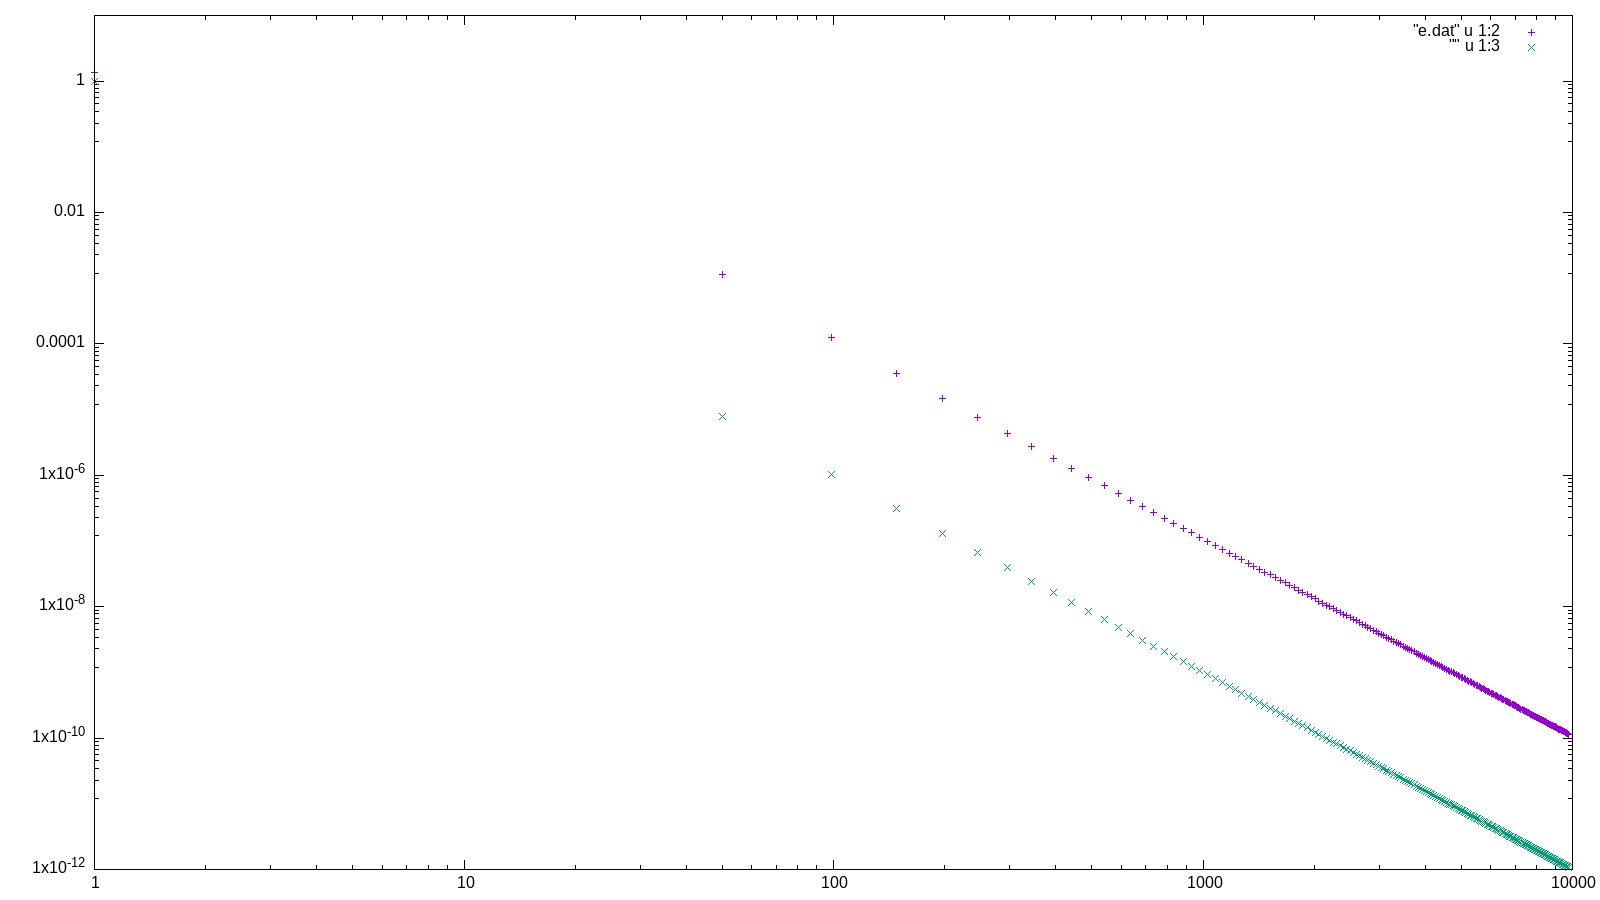
\includegraphics[width=.9\textwidth]{../fortran/BDF3_error.png}
        \end{center}
        
    \end{proof}
        

\end{enumerate}


\section*{Problem 2: Implicit/Explicit Multistep Methods for ODEs}

\begin{enumerate}[label=\alph*)]

    \item Solve the linear system,

        \begin{align}
             \Biggl\{\begin{split}
                \frac{d\bs{y}}{dt} = \bs{Ay} \\ \bs{y}(0) = \bs{y}_0
            \end{split} \\
            \bs{y}_0 = \left[\begin{array}{c}-3 \\ 1\end{array}\right], \quad &\text{and} \quad \bs{A} = \left[\begin{array}{c c}-1 & 3 \\ -3 & -1 \end{array}\right]
        \end{align}

        We solve this problem using the eigenvalues and eigenvectors of the linear system. 

        \begin{align}
            P_{\lambda}(A) &= \lambda^2 - \Tr{A}\lambda + \det(A) \\
            P_{\lambda}(A) &= \lambda^2 +2\lambda + 10 \\
            \lambda &= \frac{-2 \pm \sqrt{-36}}{2} \\
            \lambda &= -1 \pm 3i
        \end{align}

        We now solve the eigenvector problem analytically, this comes out rather obviously, 
        \begin{align}
            \lambda_1 = -1 + 3i, \quad v_1 = \left[\begin{array}{c}1 \\ i \end{array}\right] \\
            \lambda_2 = -1 - 3i, \quad v_2 = \left[\begin{array}{c}i \\ 1 \end{array}\right] \\
        \end{align}
        We then use this to write our solution.
        \begin{align}
            \bs{y}(t) &= c_1v_1e^{-t + 3it} + c_2v_2e^{-t - 3it} \\
            \bs{y}(t) &= c_1\left[\begin{array}{c}1 \\ i \end{array}\right]e^{-t}\left(\cos(3t) + i\sin(3t)\right) 
                         + c_2\left[\begin{array}{c}i \\ 1 \end{array}\right]e^{-t}\left(\cos(3t) - i\sin(3t)\right) \\
             \bs{y}(t) &= c_1\left[\begin{array}{c}1 \\ 0 \end{array}\right]e^{-t}\cos(3t) 
                        +  c_1\left[\begin{array}{c}0 \\ -1 \end{array}\right]e^{-t}\sin(3t)
                         + c_2\left[\begin{array}{c}0 \\ 1 \end{array}\right]e^{-t}\cos(3t)
                          + c_2\left[\begin{array}{c}1 \\ 0 \end{array}\right]e^{-t}\sin(3t)
        \end{align}
        We now solve for our coefficients. 
        \begin{align}
            \bs{y}(0) = c_1\left[\begin{array}{c}1\\0\end{array}\right] + c_2\left[\begin{array}{c}0\\1\end{array}\right] =
                        \left[\begin{array}{c}-3\\1\end{array}\right] \\
            c_1 = -3, \quad c_2 = 1
        \end{align}
        \begin{align}
            \bs{y}(t) &= \left[\begin{array}{c}1 \\ 0 \end{array}\right]e^{-t}\left(-3\cos(3t) + \sin(3t)\right)
                        +  \left[\begin{array}{c}0 \\ 1 \end{array}\right]e^{-t}\left(3\sin(3t) + \cos(3t)\right) \\
            \bs{y}(t) &= \left[\begin{array}{c}-3\cos(3t)+\sin(3t)\\3\sin(3t)+\cos(3t)\end{array}\right]e^{t}              
        \end{align}
        A plot of this function is shown below. 
        \begin{center}
            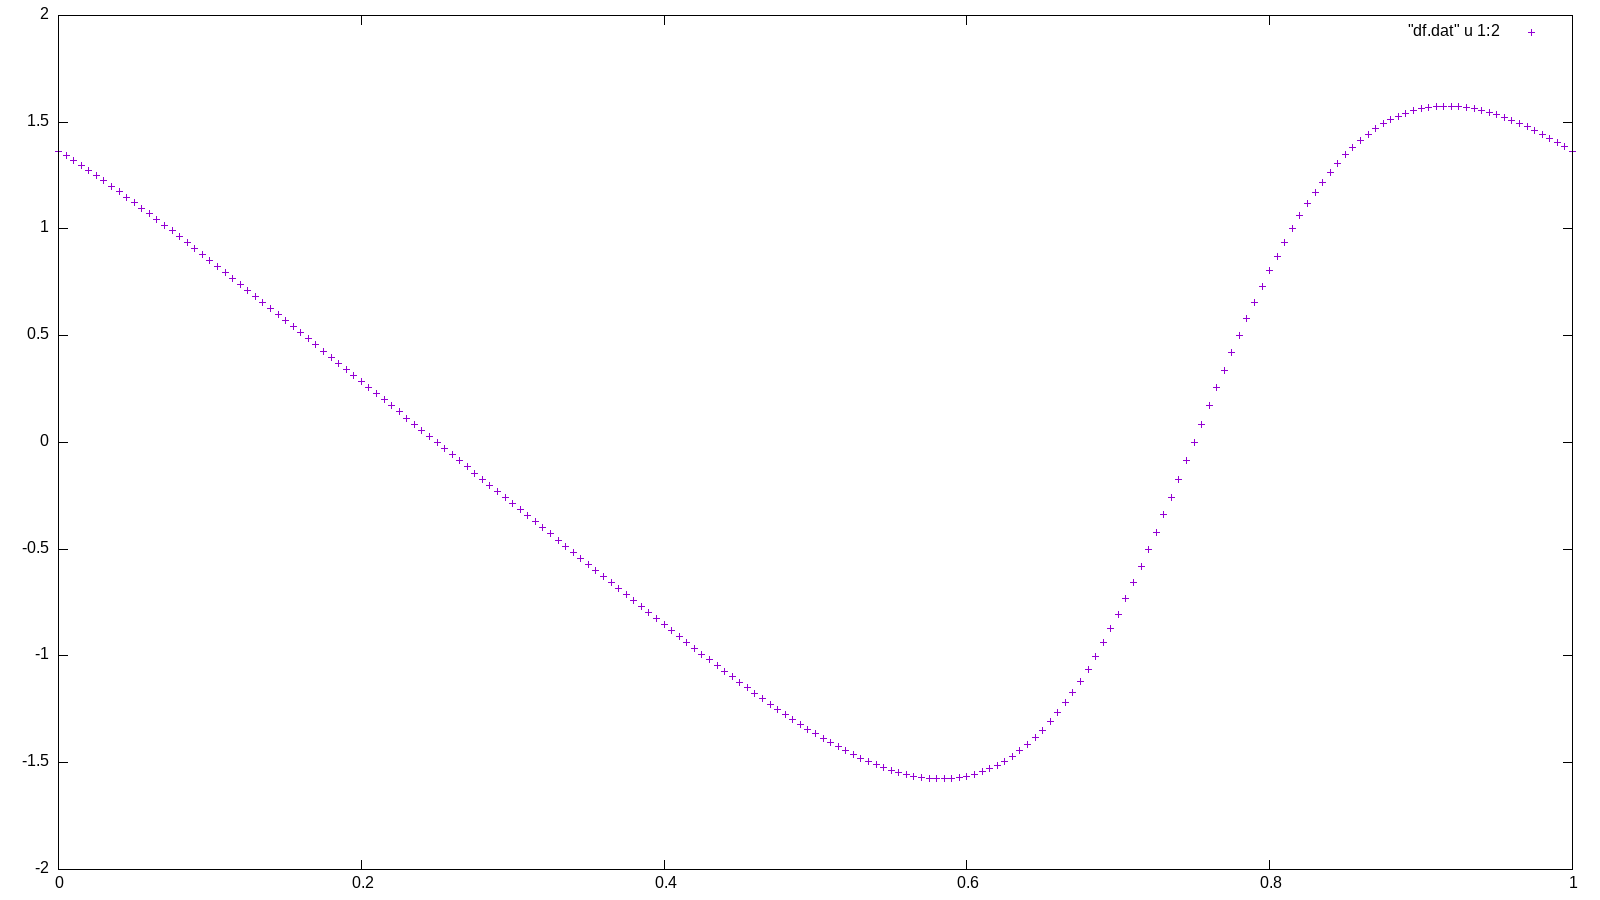
\includegraphics[width=.8\textwidth]{../fortran/question2a.png}
        \end{center}

        \item I wrote the code haha. Go see the fortran directory and see the NumDE.f90 module.

        \item We can demonstrate the exact formulations for this specific RK3 and AM3 methods. They are as follows. 
        For RK3, we have, 

        \begin{align}
            K_1 &= f(y_k) = Ay_k \\
            K_2 &= f(y_k + \frac{\Delta t}{3} K_1) = Ay_k + \frac{\Delta t}{3} A^2y_k\\
            K_3 &= f(y_k + \frac{2\Delta t}{3} K_2) = Ay_k + \frac{2\Delta t}{3} A^2y_k + \frac{2\Delta t^2}{9} A^3y_k \\
            y_{k+1} &= y_k + \Delta t \sum_{i=1}^3 b_iK_i = y_k + \frac{\Delta t}{4} K_1 + \frac{3\Delta t}{4} K_3
        \end{align}

        For AM3, we have, 
        \begin{align}
            \left(\I - \frac{9\Delta t}{24}A\right)y_{k+3}^{(0)} = y_{k+2} + \frac{\Delta t}{24}\left(19Ay_{k+2} - 5Ay_{k+1} + Ay_{k}\right) \\
            y_{k+3}^{(0)} = \left(\I - \frac{9\Delta t}{24}A\right)^{-1}\left[y_{k+2} + \frac{\Delta t}{24}\left(19Ay_{k+2} - 5Ay_{k+1} + Ay_{k}\right)\right] \\
            y_{k+3}^{(1)} = y_{k+2} + \frac{\Delta t}{24}\left(9Ay_{k+3}^{(0)} + 19Ay_{k+2} - 5Ay_{k+1} + Ay_{k}\right)
        \end{align}

        \item Here is the plot obtained for this question: 
        \begin{center}
            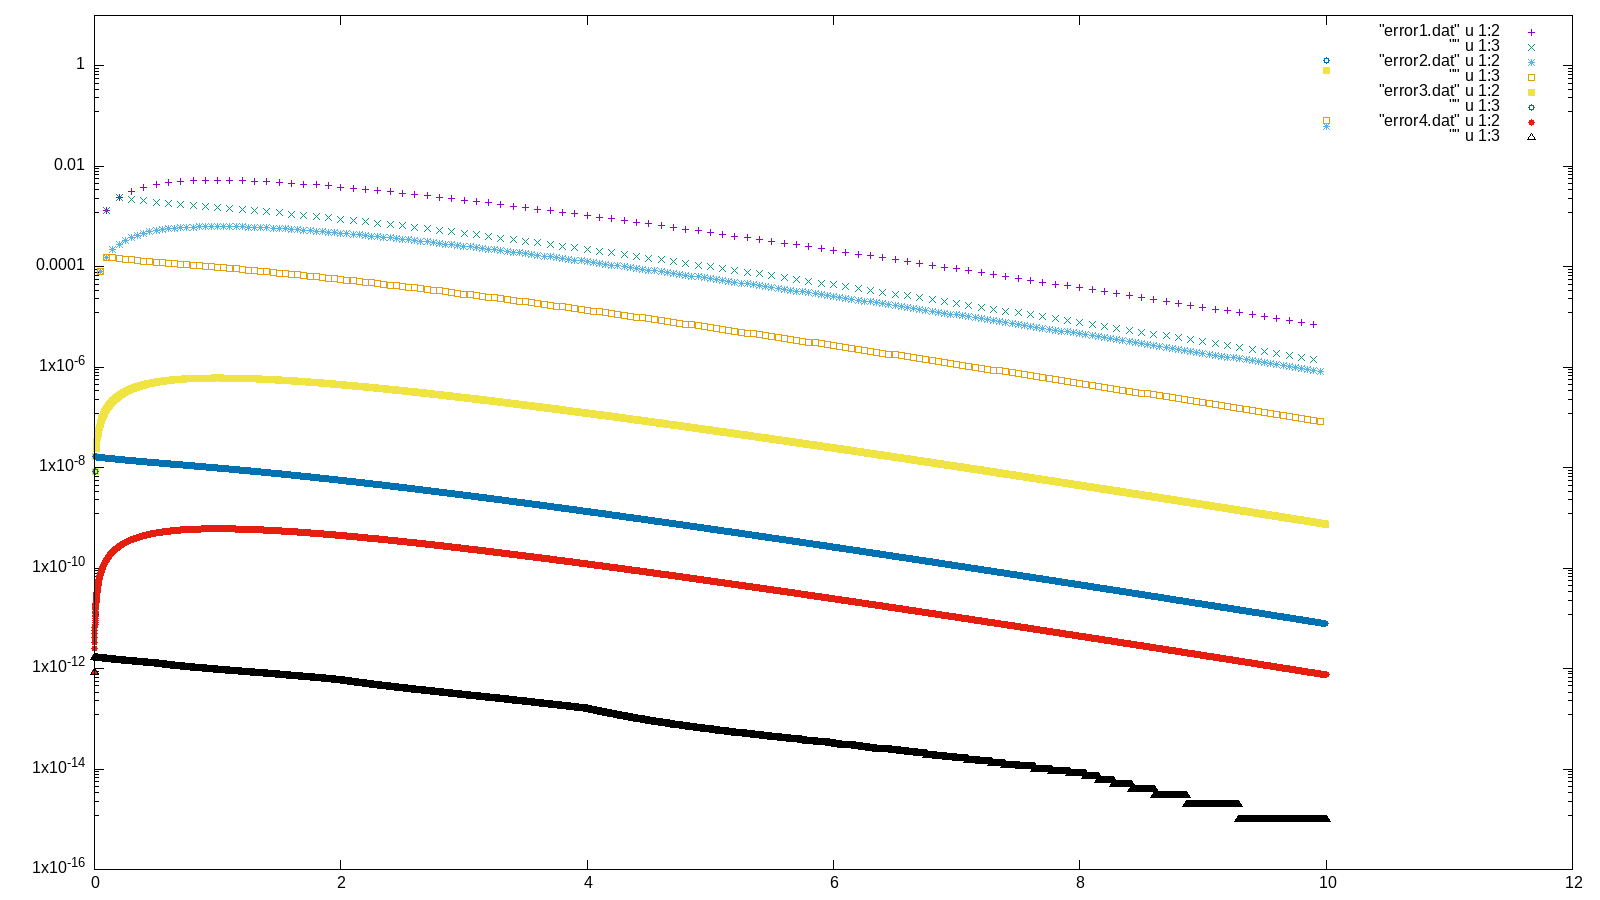
\includegraphics[width=.8\textwidth]{../fortran/error_v_t.png}
        \end{center}

        \item  The order of convergence observed for AM3 is order 4 and the order of convergence obtained for RK3 is order 3. Here is a picture of the produced plots alongside plots of order 4 and order 3 converegence for comparasion (these are plotted with lines). There are two sets of parallel lines in the plot indicating that parallel pairs have the same order of convergence. 
        \begin{center}
            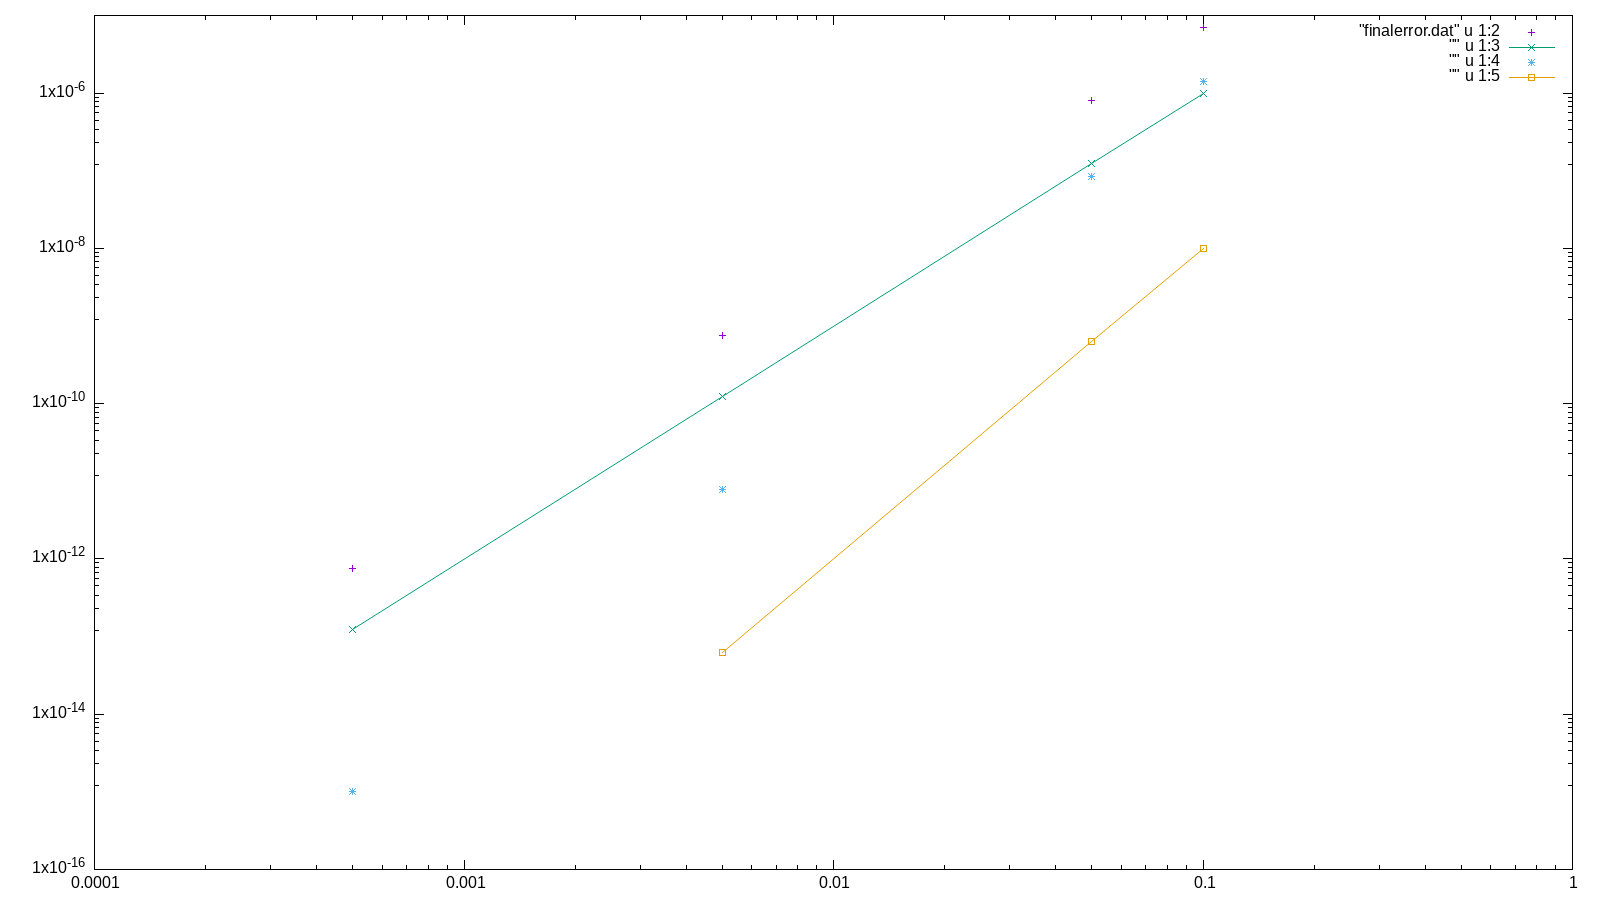
\includegraphics[width=.8\textwidth]{../fortran/final_error.png}
        \end{center}
       
       

\end{enumerate}

\end{document}
